% Created 2025-08-02 土 15:40
\documentclass[a4paper, 10pt, notitlepage, twocolumn, uplatex, oneside, dvipdfmx]{jsarticle}
\usepackage[dvipdfmx]{graphicx, color}
\usepackage{ulem}
\usepackage[utf8]{inputenc}
\usepackage{mlmodern}
\usepackage{mdframed}
\usepackage{minted}
\usepackage{natbib}
\usepackage{amsmath, amssymb, amsthm}
\definecolor{shadecolor}{gray}{0.92}
\definecolor{bgcode}{gray}{0.98}
\usemintedstyle{friendly}
\usepackage[dvipdfmx,colorlinks=true,linkcolor=blue,filecolor=blue,urlcolor=blue]{hyperref}
\usepackage{pxjahyper}
\surroundwithmdframed[backgroundcolor=shadecolor,hidealllines=true]{verbatim}
\renewcommand{\baselinestretch}{0.86}
\setlength{\voffset}{-0.7in}
\setlength{\hoffset}{-0.5in}
\setlength{\headsep}{0cm}
\setlength{\topmargin}{-0.5cm}
\setlength{\oddsidemargin}{0cm}
\setlength{\textwidth}{525pt}
\setlength{\textheight}{46\baselineskip}
\addtolength{\textheight}{\topskip}
\author{sugayu}
\date{\today}
\title{\textbf{matplotlibで作成する図の調整方法}}
\begin{document}

\maketitle
\tableofcontents

\section{基準の図}
\label{sec:org1e9be9e}
\begin{minted}[frame=lines,framesep=2mm,breaklines,bgcolor=bgcode]{ipython}
from numpy.random import default_rng
from sugayutils.figure import makefig

rng = default_rng(222)
data = rng.standard_normal(50).reshape(2, 25)


def plot_fiducial():
    fig = makefig(figsize=['small', 1.0])
    ax = fig.add_subplot(1, 1, 1)
    ax.scatter(data[0], data[1], c='blue')
    ax.set_xylabels('This is x label', 'This is y label')
    return ax

_ = plot_fiducial()
\end{minted}

\begin{center}
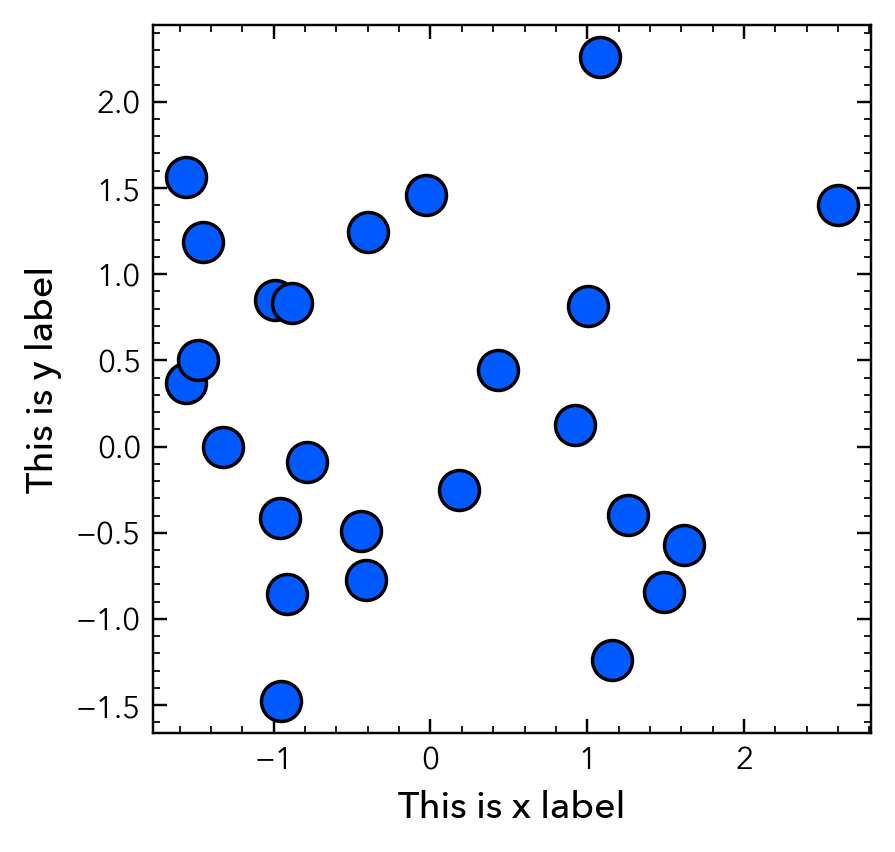
\includegraphics[width=1.0\linewidth]{./obipy-resources/fiducial.png}
\end{center}
\section{目盛り}
\label{sec:org23a9d4e}

\subsection{目盛り反転}
\label{sec:org2daefc5}
\begin{minted}[frame=lines,framesep=2mm,breaklines,bgcolor=bgcode]{ipython}
ax = plot_fiducial()
_ = ax.invert_xaxis()
\end{minted}

\begin{center}
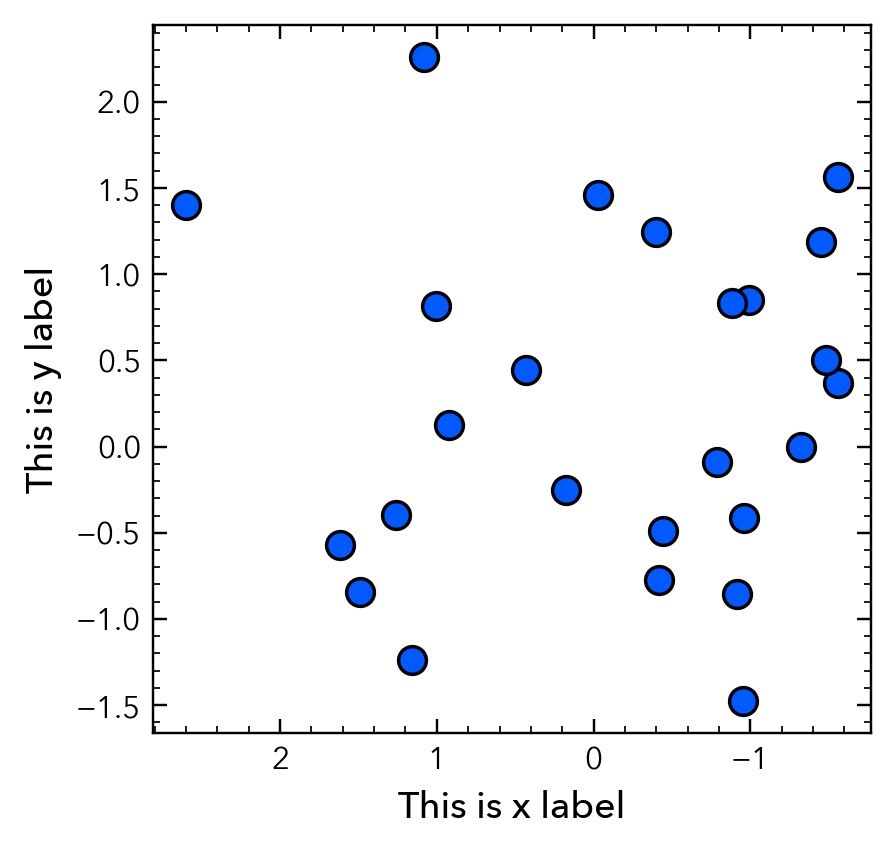
\includegraphics[width=1.0\linewidth]{./obipy-resources/params_tick_inverse.png}
\end{center}
\subsection{目盛りの数字}
\label{sec:orgd15c10c}
目盛りの情報はテキストとして格納されている。
\begin{minted}[frame=lines,framesep=2mm,breaklines,bgcolor=bgcode]{ipython}
ax = plot_fiducial()
print(ax.get_xticklabels())
plt.close()
\end{minted}

\phantomsection
\label{}
{[}Text(-2.0, 0, '−2'), Text(-1.0, 0, '−1'), Text(0.0, 0, '0'), Text(1.0, 0, '1'), Text(2.0, 0, '2'), Text(3.0, 0, '3')]

よって、このテキスト情報を変更してやればテキスト位置などを細かく変更することが可能である。
これを利用して、目盛りラベルのサイズを変更し、縦軸の目盛りを指定する。また、手作業で目盛りの位置を変更する。
\begin{minted}[frame=lines,framesep=2mm,breaklines,bgcolor=bgcode]{ipython}
ax = plot_fiducial()
ax.tick_params(labelsize='x-small') # both axes
ax.tick_params(axis='y', labelsize=20)
_ = ax.set_yticks([-0.5, 1.5, 2.0])
for i, xticklabel in enumerate(ax.get_xticklabels()):
    if i % 2 == 1:
        _, _y = xticklabel.get_position()
        xticklabel.set_y(_y - 0.05)
\end{minted}

\begin{center}
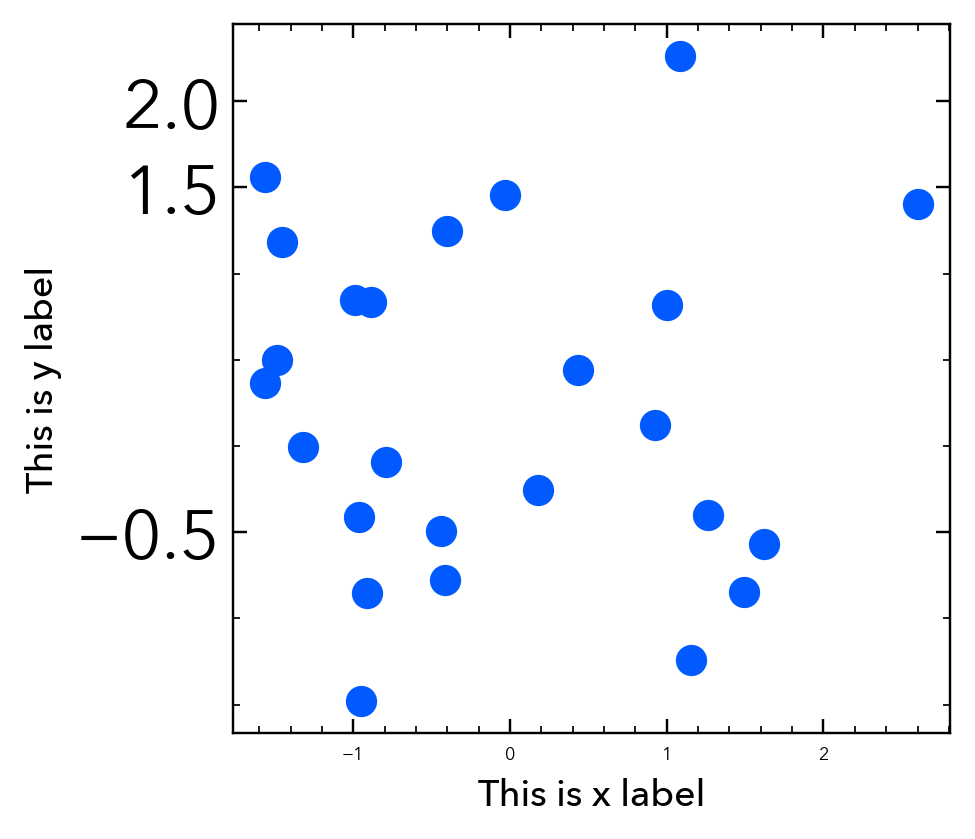
\includegraphics[width=1.0\linewidth]{./obipy-resources/params_ticks.png}
\end{center}
\section{テキスト}
\label{sec:orgdd51e1e}

\subsection{f-stringと\LaTeX{}}
\label{sec:org863de21}
f-stringと\LaTeX{}記法は併存できる。
このときf-string記法の\{\}が\LaTeX{}記法と衝突することにより、\LaTeX{}記法の\{\}に変更が加わる。
\begin{minted}[frame=lines,framesep=2mm,breaklines,bgcolor=bgcode]{ipython}
ax = plot_fiducial()
mu, sigma = 0.0, 1.0
_ = ax.text(
    *(0.1, 0.85),
    fr'logZ: $\mu_{{Z, 0}}=${mu},$\sigma_{{Z, 0}}=${sigma}',
    transform=ax.transAxes,
)
\end{minted}

\begin{center}
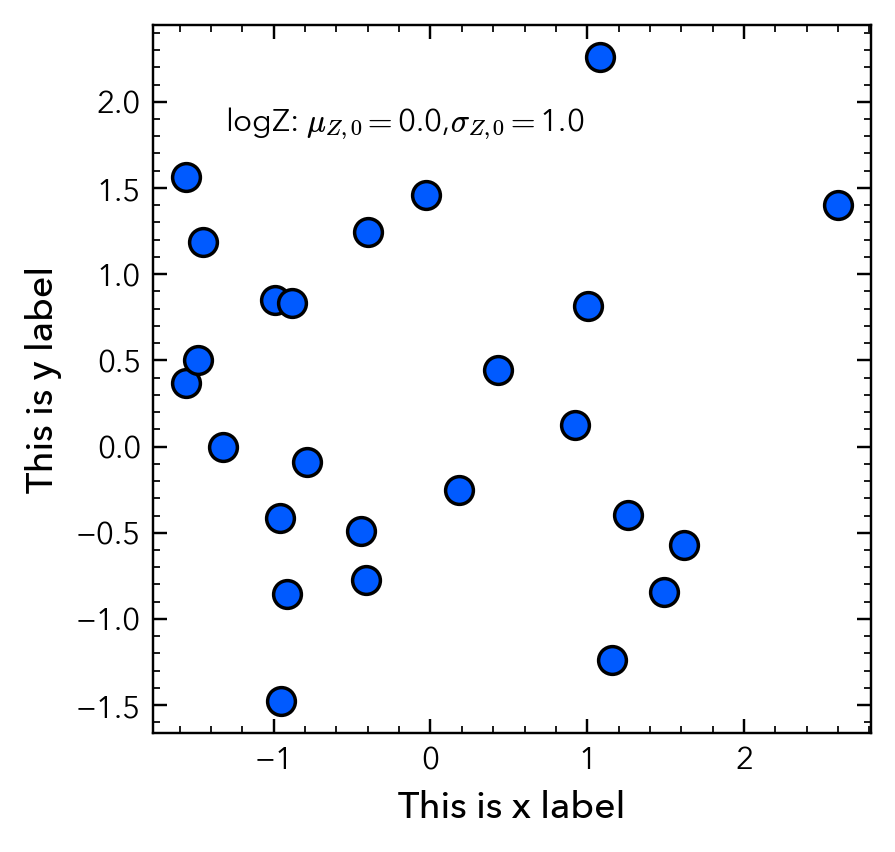
\includegraphics[width=1.0\linewidth]{./obipy-resources/params_text_fstring_latex.png}
\end{center}
\section{矢印}
\label{sec:orgd7b1a71}
\subsection{arrow}
\label{sec:org4179615}
データ座標を使って矢印を描く。
\begin{minted}[frame=lines,framesep=2mm,breaklines,bgcolor=bgcode]{ipython}
ax = plot_fiducial()
_ = ax.arrow(
    x=-1.0,
    y=-0.5,
    dx=1.0,
    dy=1.4,
    width=0.05,
    head_length=0.3,
    length_includes_head=True,
    fc='red',
)
\end{minted}

\begin{center}
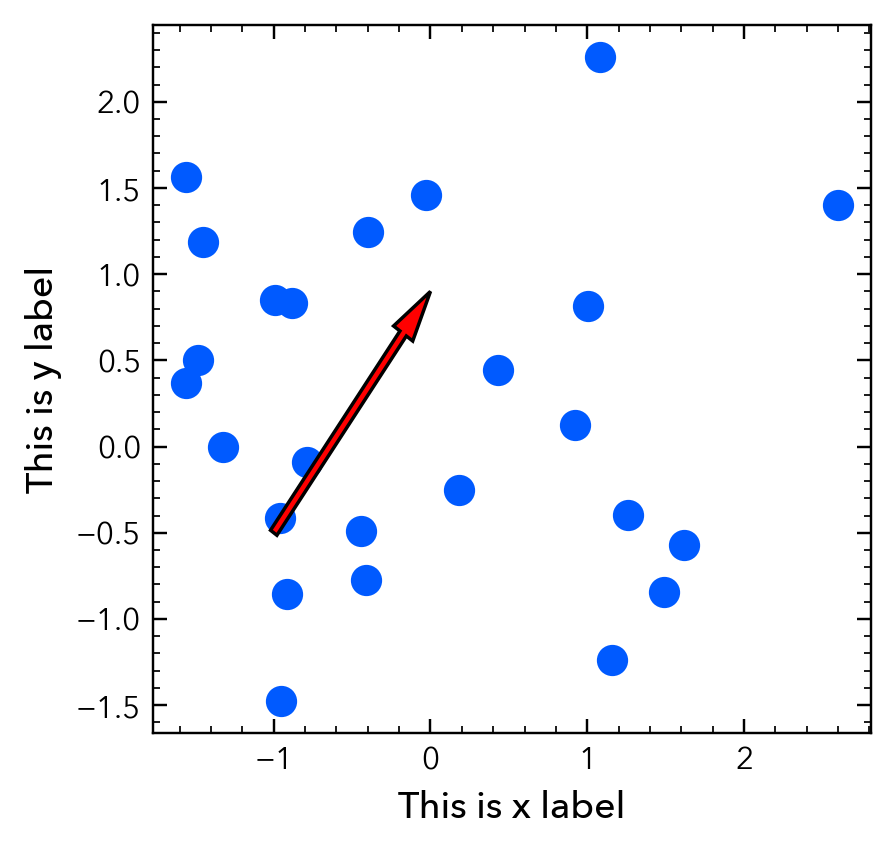
\includegraphics[width=1.0\linewidth]{./obipy-resources/params_arrow.png}
\end{center}
\section{大量の線}
\label{sec:org2127733}
一斉に同じ種類の線をプロットするには \texttt{mcoll.LineCollection} を使って、返り値を \texttt{ax.add\_collection()} で加えると良い。
\begin{minted}[frame=lines,framesep=2mm,breaklines,bgcolor=bgcode]{ipython}
import matplotlib.collections as mcoll
from sugayutils import colors

ax = plot_fiducial()
segments = (
    ((-1.0, 0.0), (1.0, 0.0)),
    ((-1.0, 0.5), (1.0, 0.5)),
    ((-1.0, 1.0), (1.0, 1.0)),
    ((-1.0, 1.5), (1.0, 1.5)),
    ((-1.0, 2.0), (1.0, 2.0)),
    ((0.0, -1.0), (0.0, 1.0)),
)
linecollection = mcoll.LineCollection(segments, colors=colors.green, lw=0.5, ls='--')
_ = ax.add_collection(linecollection)
\end{minted}

\begin{center}
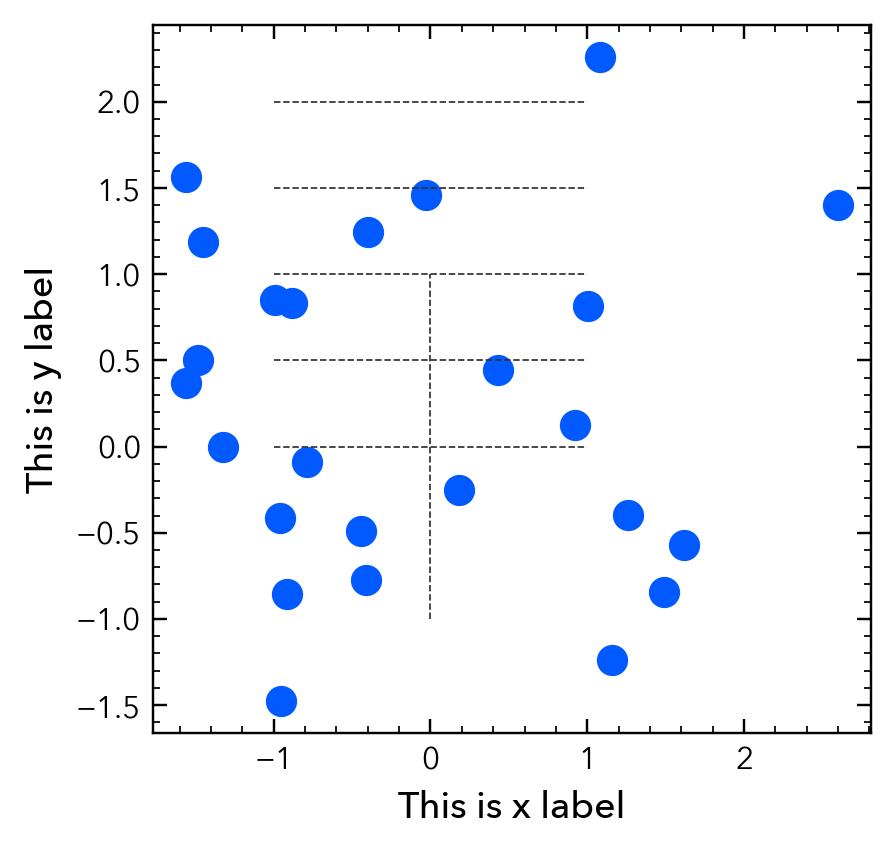
\includegraphics[width=1.0\linewidth]{./obipy-resources/params_lines.png}
\end{center}
\section{グリッド分け}
\label{sec:org1d419ec}
\texttt{fig.subplots()} と \texttt{fig.subplots\_adjust()} の組み合わせでもグリッドを切れるが、
\texttt{matplotlib.gridspec.GridSpec} を使うと引数 \texttt{width\_ratios} などを使ってより柔軟なグリッドを作ることができる。
\texttt{GridSpec} は \texttt{fig.subplots()} に引数として与えることもできるが、
\texttt{fig.add\_subplot()} で個別にパネルを作ることで \texttt{projection} などを柔軟に対応させられる。

\begin{minted}[frame=lines,framesep=2mm,breaklines,bgcolor=bgcode]{ipython}
from matplotlib.gridspec import GridSpec
gs = GridSpec(1, 2, width_ratios=(1.5, 1))
fig = plt.figure(figsize=[7.2, 3.5])
ax0 = fig.add_subplot(gs[0])
ax1 = fig.add_subplot(gs[1], projection='3d')
ax0.scatter(data[0], data[1], c='blue')
ax0.set_xlabel('This is x label')
ax0.set_ylabel('This is y label')
_ = ax1.plot(np.arange(0., 10.0), np.arange(0., 10.0), np.arange(0., 10.0))
\end{minted}

\begin{center}
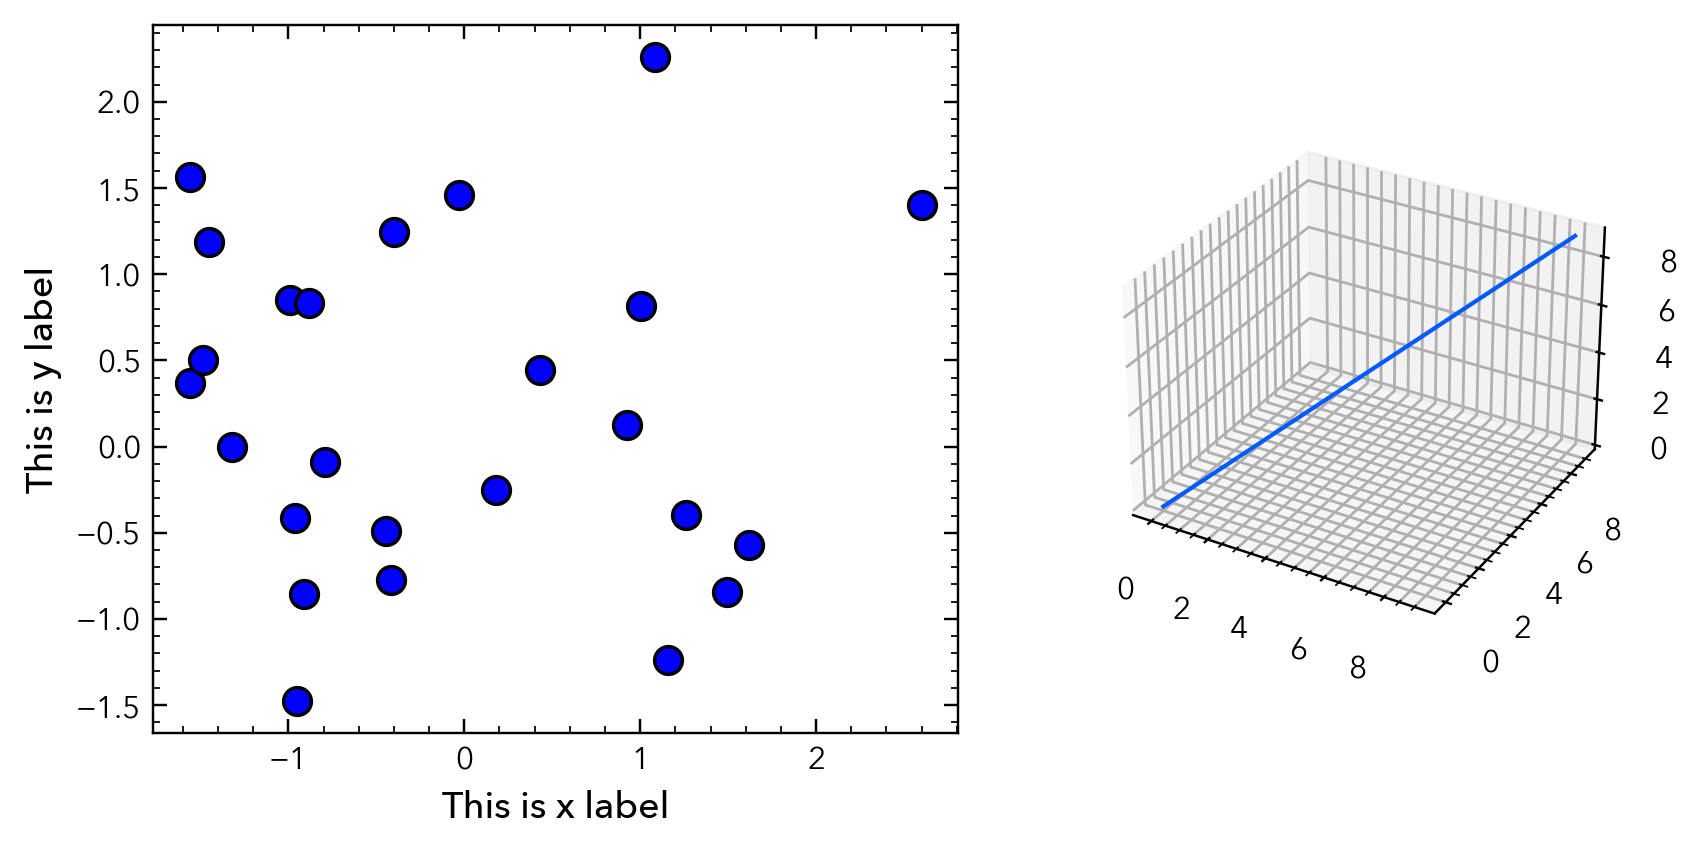
\includegraphics[width=1.0\linewidth]{./obipy-resources/params_grids.png}
\end{center}

参照: \href{https://stackoverflow.com/questions/10388462/matplotlib-different-size-subplots}{python - Matplotlib different size subplots - Stack Overflow}
\section{図}
\label{sec:org38da2c8}
\subsection{Nonuniform image}
\label{sec:org55dbc1e}
ピクセルの形が長方形になるような、各列や行によってピクセル幅が異なる画像を作成する際には
\texttt{NonUniformImage} を使う。
\texttt{ax.imshow} は画像(Image)を定義する以外に\href{https://github.com/matplotlib/matplotlib/blob/v3.10.5/lib/matplotlib/axes/\_axes.py\#L5750-L5996}{内部で様々な設定を同時にしてくれている}が、
\texttt{NonUniformImage} を使う場合には自分で画像の設定をする必要がある。
例えば、以下の例では \texttt{extent} 自体は \texttt{NonUniformImage} を呼ぶ際に設定しているが、
画像の縦横サイズ \texttt{xlim} と \texttt{ylim} は自動では設定されないので、
 \texttt{im.set\_extent()} を明示的に呼ぶことで \texttt{extent} に合わせて画像サイズを設定している。

\begin{minted}[frame=lines,framesep=2mm,breaklines,bgcolor=bgcode]{ipython}
from matplotlib.image import NonUniformImage

fig = makefig(figsize=['small', 0.6])

x = (np.arange(15) - 7.0)
x = x**3 / 7.0**3 * 3.0
y = (np.arange(9) - 4.0)
image = np.exp(-0.5 * (x[None, ...]**2 + y[..., None]**2))
extent = (-3.5, 3.5, -4.5, 4.5)
kw = dict(
    extent=extent,
    origin='lower',
    cmap='YlGn',
)

ax = fig.add_subplot(1, 2, 1)
im = NonUniformImage(ax, interpolation='nearest', **kw)
im.set_data(x, y, image)
im.set_extent(extent)
ax.add_image(im)
ax.set_aspect('auto')

ax = fig.add_subplot(1, 2, 2)
ax.imshow(image, aspect='auto', **kw)
_ = ax.set_title('Uniform (worng scale)')
\end{minted}

\begin{center}
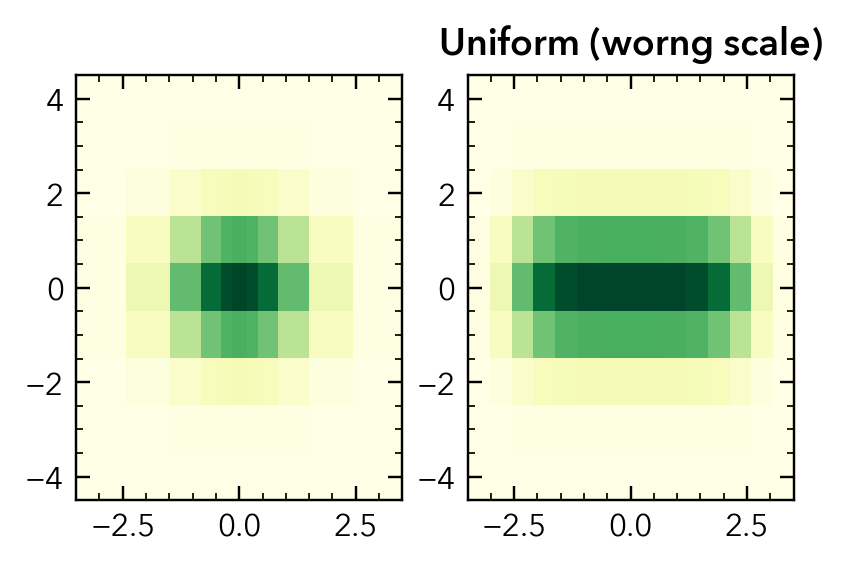
\includegraphics[width=1.0\linewidth]{./obipy-resources/params_image_nonuniformimage.png}
\end{center}

\begin{itemize}
\item \href{https://matplotlib.org/stable/gallery/images\_contours\_and\_fields/image\_nonuniform.html}{Image nonuniform — Matplotlib 3.10.5 documentation}
\end{itemize}
\end{document}
